\documentclass[12pt, a4paper]{report}
\usepackage{amsmath}  % 数学符号支持
\usepackage{amssymb}  % 额外数学符号支持
\usepackage{graphicx} % 图形支持
\usepackage{setspace}
\setstretch{1.5}
\usepackage{biblatex}
\usepackage{graphicx}
\usepackage{float}
\graphicspath{ {image/}} %image为文件夹名,可以在左侧自己创建文件夹
\addbibresource{reference.bib}
\begin{document}

% 封面页
\begin{titlepage}
    \centering
    \vspace*{1cm}
    
    {\LARGE \textbf{Collision-free Navigation of Wheeled Mobile Robots in Complex Environment}}
    
    \vspace{1.5cm}
    
    \textbf{Author Name: Zichen Zhang}\\
    \textbf{Student ID: z5490421}\\
    \vspace{0.5cm}
    
    Thesis submitted as a requirement for the degree\\
    Bachelor of Engineering (Electrical Engineering)\\
    
    \vfill
    
    School of Electrical Engineering and Telecommunications\\
    University of New South Wales\\
    
    \vspace{0.8cm}
    
    \textbf{Supervisor: Andrey V. Savkin}
    
    \vspace{1.5cm}
    
    Submission Date: November 14, 2024
    
\end{titlepage}

% 生成目录
\tableofcontents
\newpage

% 后续章节可以在此添加
\begin{abstract}
    This thesis investigates the problem of collision-free navigation for wheeled mobile robots in complex environments. With the growing demand for autonomous systems capable of safely navigating dynamic and unpredictable settings, more efficient and practical navigation algorithms have been developed. This thesis focuses on one such navigation algorithm—the Sliding Mode Control (SMC)—to test and analyze its principles and evaluate its performance through simulation results to determine its efficiency.
\end{abstract}


\chapter{Background}
Navigation of mobile robots in complex environments has always been a critical topic in the field of robotics research. Such environments often involve static and dynamic obstacles, uneven terrain, and various operational uncertainties. To address these challenges, numerous efficient navigation algorithms have been developed worldwide, finding applications across industries such as industrial automation, autonomous transportation, and surveillance. In this chapter, I will introduce some classical navigation algorithms.

The classical VO method, proposed by Fiorini and Shiller, determines safe trajectories by analyzing the relative velocities between obstacles and the robot \cite{Fiorini1998}, provides a foundation for dynamic collision avoidance in 2D spaces. Recent advances extend this method to three-dimensional scenarios, allowing safe navigation of unmanned aerial vehicles in cluttered airspaces \cite{Bareiss2015}.

Model Predictive Control (MPC) has emerged as a highly effective strategy. By continuously optimizing control inputs over a finite horizon, MPC facilitates real-time trajectory planning while ensuring stability \cite{Mayne2014}. Approaches like Tube MPC, which fall under robust MPC strategies, are well-suited for uncertain environments due to their ability to incorporate error bounds, ensuring the maintenance of stable and reliable trajectories \cite{Mayne2014}.

The Artificial Potential Field (APF) method is a popular reactive navigation technique that uses a virtual field to guide robots toward their targets. In this field, obstacles generate repelling forces, while the target exerts an attractive force \cite{Kim2000}. Enhancing its practical use, researchers have incorporated kinematic constraints, making it more suitable for real-world robotic applications \cite{Ge2000}.

The Bug algorithm is also a strategy for navigation in unknown environments. These algorithms rely on local sensing to avoid obstacles while ensuring progress toward the goal. Their simplicity and guaranteed convergence make them ideal for robots with limited computational resources \cite{Lumelsky1991}. The classic Bug1 and Bug2 algorithms have been enhanced to improve efficiency and adaptability in dynamic and cluttered settings \cite{Lumelsky1991}.

In multirobot systems, coordination becomes critical for efficient and collision-free operation. Distributed MPC has emerged as a promising approach, enabling robots to optimize their trajectories collaboratively while taking into account the constraints of other robots in the environment \cite{Turpin2014}. Furthermore, augmented Lagrangian decomposition techniques have been employed to achieve scalable decentralized navigation in large robotic teams \cite{Dunbar2006}.

 A comprehensive comparison of these algorithms is presented in a table from the work of Hoy, Matveev, and Savkin \cite{Hoy2015}, which categorizes different methods based on their applicability to specific scenarios such as single vehicle navigation, avoidance of moving obstacles, coordination of multiple vehicles, and boundary following.

 \begin{figure}[H]
    \centering
    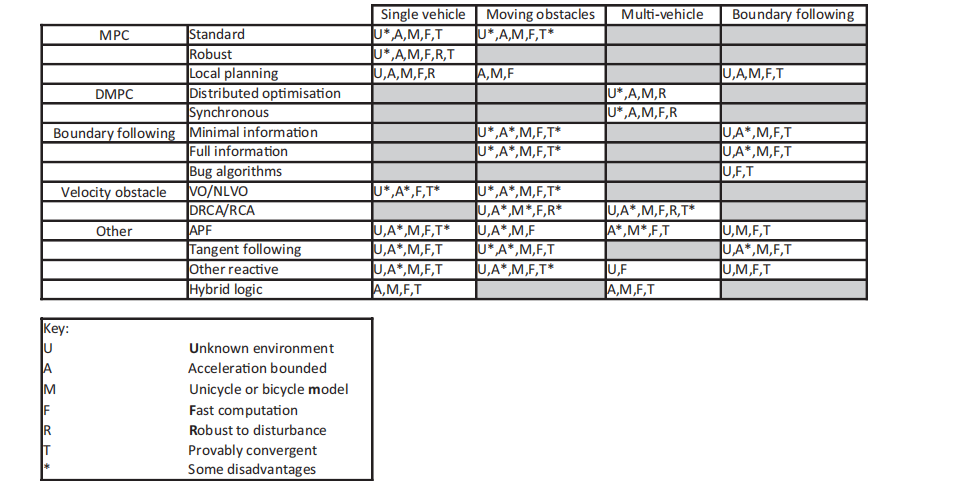
\includegraphics[width=0.8\textwidth]{11.png}
    \caption{compares the applicability of various algorithms discussed in \cite{Hoy2015}}
    \label{FIG:11}
\end{figure}

This paper focuses on discussing the operational strategy of the Sliding Mode Control (SMC) method and testing its performance in various obstacle scenarios. The strategy will be evaluated at the end of the paper.

% 包含 Methodology 文件
\chapter{Methodology}

\section{Introduction to Sliding Mode Control}

Sliding Mode Control (SMC) is a well-established strategy within the broader category of sensor-based control techniques. It is recognized for its robustness in maintaining system stability, even when confronted with uncertainties and external disturbances\cite{Hoy2015}.Fundamentally, SMC belongs to a specific class of nonlinear control methods, with its distinctiveness arising from the discontinuity inherent in its control signals. By continually adjusting the sliding surface based on the system's real-time state, SMC compels the system to adhere to a predefined ``sliding mode'' trajectory. This capability ensures precise control over the system's behavior throughout the process. Additionally, SMC dynamically adapts the control input through feedback mechanisms, enabling the system to remain stable and consistently follow the desired trajectory, even under significant external perturbations \cite{Liu2012}.The sliding surface is a crucial concept in the entire strategy.


\section{Definition of the Sliding Surface}
Consider a general scenario where, in the system 
\[
\dot{x} = f(x), \quad x \in \mathbb{R}^n,
\]
there is a switching surface 
\[
s(x) = s(x_1, x_2, \dots, x_n) = 0.
\]

This switching surface divides the state space into two distinct regions: \(s > 0\) and \(s < 0\). The system's behavior in the vicinity of this surface can be categorized into three distinct cases, as illustrated in Figure \ref{FIG:1}.



\begin{figure}[H]
    \centering
    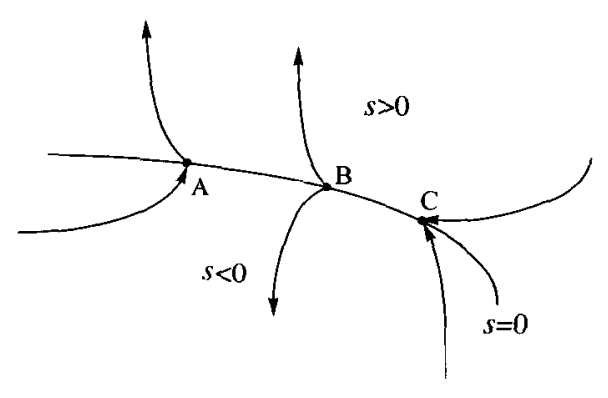
\includegraphics[scale=0.5]{1.png}
    \caption{Sliding Surface} % 图名称
    \label{FIG:1}
\end{figure}

The system trajectory demonstrates three unique types of behavior in proximity to the switching surface, where \(s = 0\).


1. \textbf{Regular Point}: The trajectory of the system moves toward the switching surface \( s = 0 \) and crosses through it, as represented by Point A.

2. \textbf{Starting Point}: The trajectory of the system approaches the switching surface \( s = 0 \) from both sides, converging to the surface without actually crossing it. This behavior is depicted by Point B.

3. \textbf{Endpoint}: The trajectory of the system reaches the switching surface \( s = 0 \) and remains on it, approaching from both sides without departing from the surface. This is illustrated by Point C.

    In sliding mode control, the starting point typically holds little significance, while the terminal point is of special importance. This is because once the system state point enters a particular region on the switching surface, all points within this region are considered terminal points. As the state point approaches this region, it is "attracted" to and remains within it. This region, located at \( s=0 \), is referred to as the "sliding mode region" or simply the "sliding region." The motion of the system within this region is known as "sliding motion."

 According to the sliding mode control requirements, all points in the sliding region should be treated as terminal points. When the system state approaches the switching surface \( s(x) = 0 \), it must satisfy the following conditions:
\begin{equation}
\lim_{\dot{s} \to 0^+} \dot{s} \leq 0 \quad \text{and} \quad \lim_{\dot{s} \to 0^-} \dot{s} \geq 0.
\label{eq:sliding_conditions}
\end{equation}
 For the controller in the sliding mode control algorithm, the primary objective is to ensure that the system state meets the conditions of the sliding surface. Under the control law of the sliding mode control method described below, the vehicle's initial control input is set to an extreme value to ensure that the system state quickly converges to the sliding surface.

\subsection{Dynamics and State Space of the Mobile Robot}

In implementing the Sliding Mode Control (SMC) method, we first define the dynamics and state space of the mobile robot to capture its kinematic behavior accurately. Based on the work by Matveev et al. \cite{Matveev2012}, the mobile robot is modeled as a planar underactuated nonholonomic system, similar to a unicycle model.

The robot's state space can be defined as \( \mathbf{x} = [x, y, \theta]^T \), where:
- \( x \) and \( y \) represent the position of the robot in the Cartesian plane,
- \( \theta \) is the orientation angle of the robot with respect to a reference axis.

The dynamics of the mobile robot are governed by the following equations:

\begin{equation}
\dot{x} = v \cos \theta
\end{equation}
\begin{equation}
\dot{y} = v \sin \theta
\end{equation}
\begin{equation}
\dot{\theta} = u
\end{equation}

where \( v \) is the constant linear velocity, and \( u \) is the control input representing the angular velocity. \( u \) is limited by \( u \in [-\bar{u}, \bar{u}] \), ensuring that the angular velocity does not exceed a maximum threshold \( \bar{u} \).

\subsection{Boundary Following Sliding Mode Control Law}

The core of the sliding mode strategy is to ensure that the robot maintains a predefined distance from the nearest obstacle at all times. When \( d(t) \) becomes smaller than the predefined parameter (indicating proximity to the obstacle), the switching function rapidly drives the robot away. The operational logic of this strategy will be explained in detail through the following equations.

\subsubsection*{Distance Calculation}
The distance between the vehicle's current position \(r(t) = \text{col}(x(t), y(t))\) and the domain \(D\) is mathematically defined as:
\[
d(t) := \text{dist}_D[r(t)] = \min_{r' \in D} \|r - r'\|,
\]
where \(r = \text{col}(x, y)\) and \(r' = \text{col}(x', y')\). The Euclidean norm \(\|\cdot\|\) is represented as:
\begin{equation}
\| r - r' \| := \sqrt{(x - x')^2 + (y - y')^2}
\label{eq:euclidean_norm}
\end{equation}
This definition ensures that \( d(t) \) represents the shortest distance between the vehicle and the boundary of domain \( D \).

\textbf{Control Law}
To drive the vehicle towards the target boundary distance \( d_0 \), the following discontinuous control law is applied:
\begin{equation}
u(t) = \bar{u} \cdot \text{sign}\{\dot{d}(t) + \chi[d(t) - d_0]\}
\label{eq:control_law}
\end{equation}
where \( \bar{u} \) represents the maximum allowable angular velocity, and \( \chi(z) \) is defined as:
\begin{equation}
\chi(z) := \begin{cases} 
      \gamma z & \text{if } |z| \leq \delta \\
      v_* \cdot \text{sign}(z) & \text{if } |z| > \delta 
   \end{cases}
\label{eq:chi_definition}
\end{equation}

In this context, the sign function \(\text{sign}(\alpha)\) is defined such that \(\text{sign}(\alpha) = 1\) when \(\alpha > 0\), \(\text{sign}(0) = 0\), and \(\text{sign}(\alpha) = -1\) for \(\alpha < 0\). The parameters \(\gamma > 0\) and \(\delta > 0\) represent control constants, while \(v_\ast := \gamma \delta\) denotes the upper bound for the control output when \(|z|\) exceeds \(\delta\).

The basic functions of sliding mode control design were summarized above. With an understanding of the fundamental principles, this paper will proceed to conduct relevant environmental tests for this type of controller.


\section{Evaluation of SMC in Various Environments}

The practical implementation of the Sliding Mode Control (SMC) method is presented in this paper by evaluating the performance and implementing tests on a wheeled robot under several scenarios as further chapters. These test scenarios are broken down into the following categories to simulate complex real-world conditions:

\begin{itemize}
    \item \textbf{Simulation of Static Obstacles Avoidance}: This scenario evaluates the controller's ability to maintain a safe distance while avoiding static obstacles, without a specific target. The vehicle's movement trajectory is observed during the process.

    \item \textbf{Simulation of Moving Obstacles Avoidance}: This scenario assesses the controller's ability to maintain a safe distance while avoiding dynamic obstacles, without a specific target. The vehicle's movement trajectory is analyzed to evaluate its obstacle avoidance capabilities.

    \item \textbf{Target Navigation in a Static Obstacle Environment}: This scenario is designed with multiple static obstacles, and a predefined target for the robot to reach. The test aims to evaluate the balance achieved by the Sliding Mode Control method between effective obstacle avoidance and efficient path planning.

    \item \textbf{Target Navigation in a Dynamic Obstacle Environment}: This scenario includes multiple dynamic obstacles that move unpredictably relative to the robot. The robot is required to adjust its path quickly while pursuing the target and reach the predefined goal. The primary aim of this test is to assess the robustness and real-time responsiveness of the Sliding Mode Controller.
\end{itemize}

By analyzing the robot's performance in static and dynamic environments, these experiments aim to comprehensively evaluate the Sliding Mode Controller's effectiveness under various conditions.


\chapter{Experiment}

This chapter primarily discusses the trajectory performance of the robot in different test scenarios, detailing the parameters of both the controller and the robot. Additionally, this chapter provides a brief evaluation of the accuracy and applicability of the SMC controller under various test conditions.

\section{Experimental Setup}

In this section, we outline the relevant parameters and simulation environment used in the experiment:
\begin{itemize}
    \item \textbf{Vehicle Parameters}: Provide details about the simulated vehicle model, including maximum speed(), maximum angular velocity, turning radius, initial coordinates, and initial angle.

    \item \textbf{SMC Parameters}: List the key parameters for the SMC controller, such as the control gain \( \gamma \), boundary distance \( d_{\text{safe}} \), and switching thresholds \( \delta \).
    \item \textbf{Simulation Environment}: Describe the simulation tools (e.g., MATLAB) and settings, including grid size, time steps, and visualization setup.
\end{itemize}

\section{Testing Scenarios}

Each of the following test scenarios represents a different type of environment to evaluate the SMC controller's effectiveness in navigation tasks.

\subsection{Simulation of Static Obstacles Avoidance}
In this scenario, stationary point obstacles are placed at fixed coordinates \((1, 1)\), \((2, 2)\), and \((3, 3)\) within a bounded simulation environment. The mobile robot is initialized at the origin \((0, 0)\) with a heading angle of \(0\), facing the positive \(x\)-axis. The obstacles are modeled as point objects with no dynamic behavior, allowing the robot to focus solely on path planning and avoidance using the sliding mode control algorithm.

The simulation parameters are set as follows: the robot maintains a constant linear velocity of \(1\,\text{m/s}\) and adjusts its angular velocity based on the sliding mode control law, with a maximum angular velocity \(u_{\text{max}} = 1.5\,\text{rad/s}\). The safety distance \(d_{\text{safe}} = 2\,\text{m}\) ensures the robot remains sufficiently clear of obstacles throughout the trajectory. The controller parameters \(\gamma = 2\) and \(\delta = 2\) are chosen to balance the responsiveness and stability of the sliding mode control, while \(v_\ast = \gamma \cdot \delta = 4\) defines the maximum adjustment for \(\chi(z)\) in the nonlinear control region.

The robot navigates the environment by continuously monitoring the distance \(d(t)\) to the closest obstacle and computing the rate of change of distance \(\dot{d}(t)\) using numerical differentiation. The sliding mode control law governs the angular velocity \(u(t)\) as:
\begin{equation}
u(t) = u_{\text{max}} \cdot \text{sign} \left( \dot{d}(t) + \chi[z(t)] \right),
\end{equation}
where \(z(t) = d(t) - d_{\text{safe}}\) and the auxiliary function \(\chi(z)\) is defined as:
\begin{equation}
\chi(z) =
\begin{cases}
\gamma \cdot z, & \text{if } |z| \leq \delta, \\
v_\ast \cdot \text{sign}(z), & \text{if } |z| > \delta.
\end{cases}
\end{equation}

During the course of \(200\) simulation steps (\(20\,\text{s}\) total simulation time, with a time step of \(0.1\,\text{s}\)), the robot's trajectory is recorded and analyzed. The results demonstrate the robot's ability to successfully navigate the environment while maintaining a safe distance from all obstacles. The trajectory is visualized in Figure \ref{FIG:2}, where the robot's path is represented by a red line, and obstacles at stationary points are marked as red "×" symbols.

\begin{figure}[H]
    \centering
    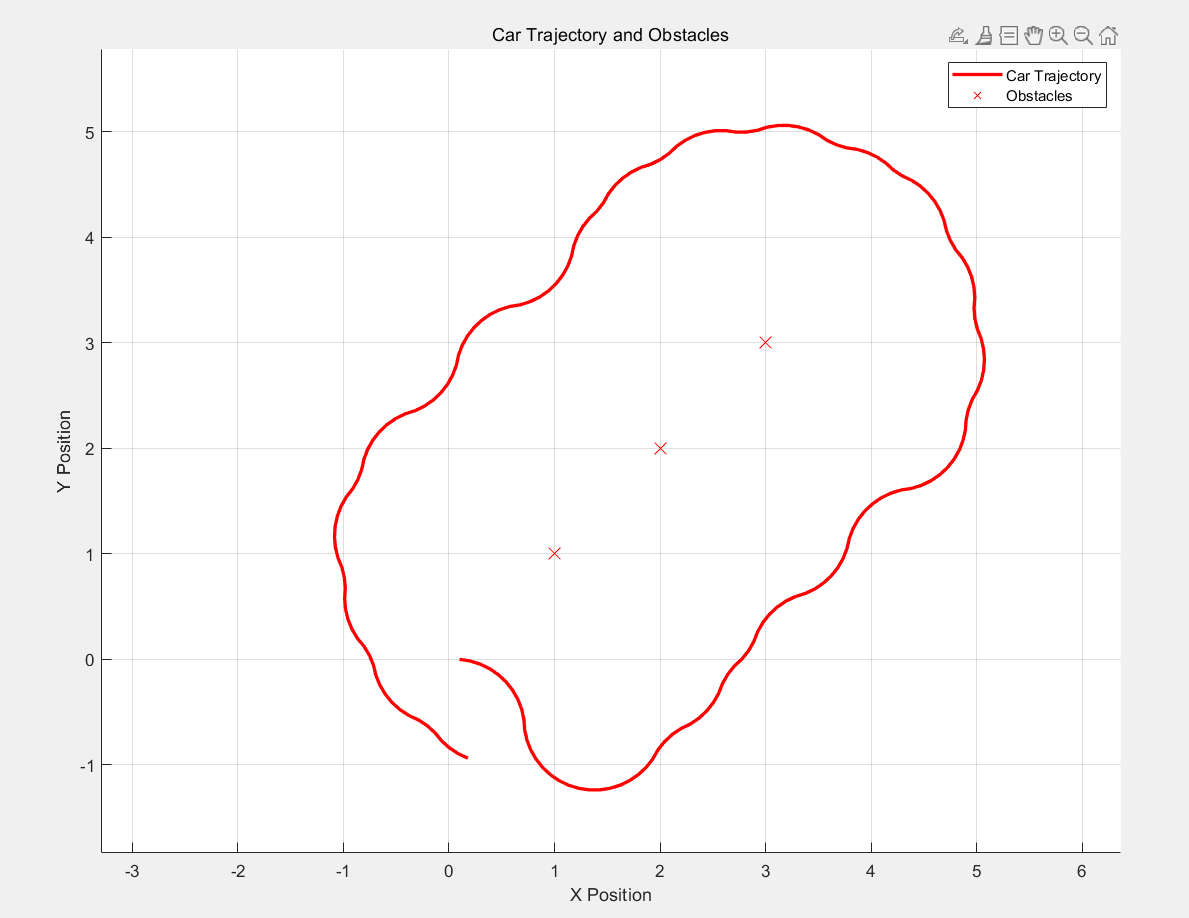
\includegraphics[scale=0.5]{2.png}
    \caption{Car Trajectory} % 图名称
    \label{FIG:2}
\end{figure}

The temporal evolution of the distances between the robot and each obstacle is illustrated in Figure \ref{FIG:3}. Each curve corresponds to a specific obstacle, showing how the robot dynamically adjusts its trajectory to maintain a safe distance. At the start of the simulation, the robot rapidly approaches the nearest obstacle, causing the corresponding distance curve to decrease. Once the robot reaches the minimum allowable distance (\(d_{\text{safe}} = 2 \, \text{m}\)), the sliding mode controller adjusts its motion to maintain the safety threshold while maneuvering around the obstacle.

\begin{figure}[H]
    \centering
    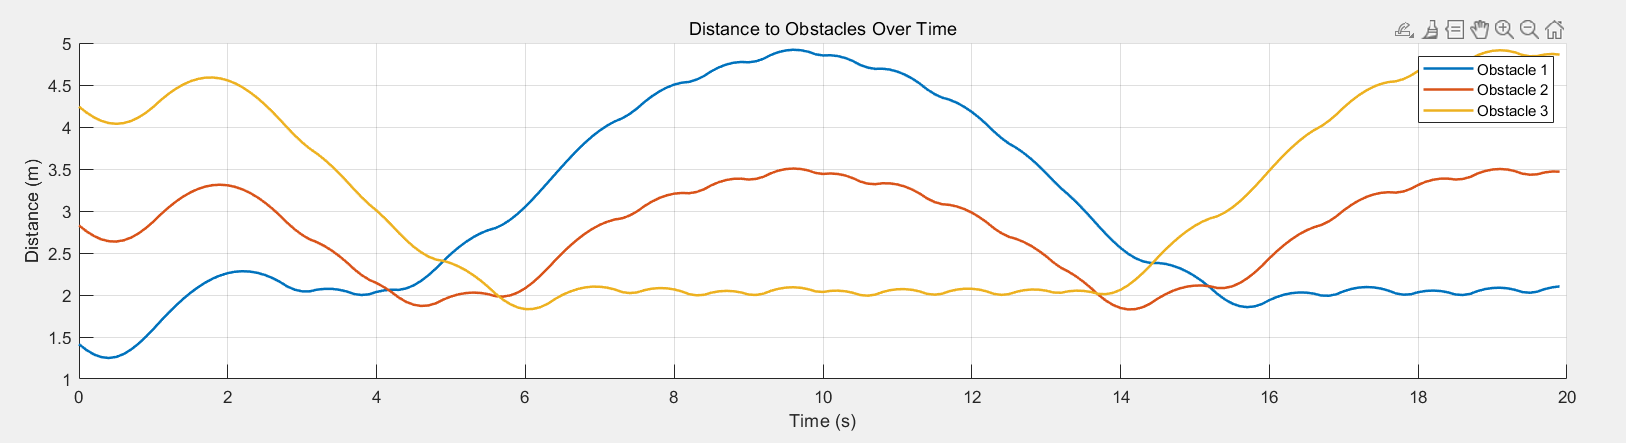
\includegraphics[width=0.8\textwidth]{3.png}
    \caption{Robot-Obstacle Distance Profiles}
    \label{FIG:3}
\end{figure}

Based on the distance graph in Figure~\ref{FIG:3}, it can be observed that the curve exhibits irregular oscillations, reflecting the robot's dynamic adjustments (sgn function) as it transitions between the influence regions of multiple obstacles. This also demonstrates the real-time responsiveness of the sliding mode control algorithm. Notably, the distance curve rarely falls below the predefined safety threshold. For instance, as shown in the figure, the orange curve remains above the set safety threshold while approaching Obstacle 3 during the 6-14 time units.

This analysis supports the effectiveness of the SMC control algorithm in maintaining safe navigation in environments with multiple static obstacles.



\subsection{Simulation of Moving Obstacles Avoidance}


\subsubsection{Initial Setup and Motion Description}


To investigate the obstacle avoidance performance of the Sliding Mode Control (SMC) algorithm under dynamic obstacles, four moving obstacles are introduced in this environment.

\begin{itemize}
    \item \textbf{Ob1}: Initial position \((2, 2)\), moving with velocity \((0.1, 0)\) m/s.
    \item \textbf{Ob2}: Initial position \((1, 2)\), moving with velocity \((-0.1, 0.1)\) m/s.
    \item \textbf{Ob3}: Initial position \((3, 3)\), moving with velocity \((0.1, -0.1)\) m/s.
    \item \textbf{Ob4}: Initial position \((4, 4)\), moving with velocity \((0.2, 0.1)\) m/s.
\end{itemize}

Detailed information about the obstacles and the initial position of the robot can be found in Figure~\ref{FIG:4}. In the figure, the robot's initial position is represented by a green circle, and the direction of motion for each obstacle is indicated with arrows.

\begin{figure}[H]
    \centering
    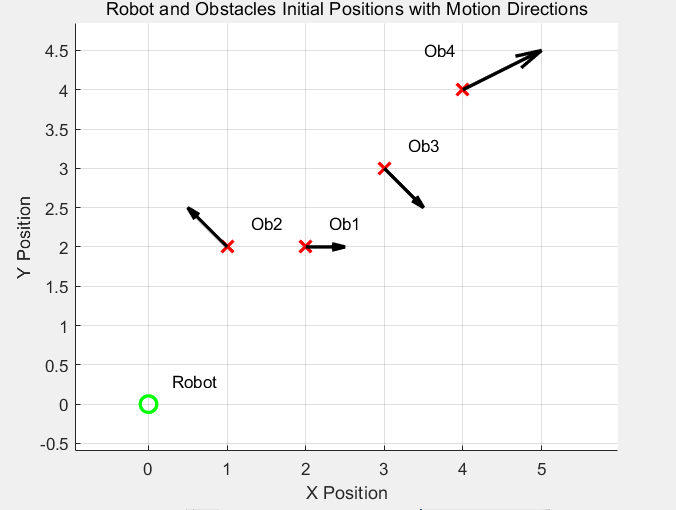
\includegraphics[width=0.8\textwidth]{4.png}
    \caption{Initial Positions and Motion Directions of Robot and Obstacles}
    \label{FIG:4}
\end{figure}

\subsubsection{Robot and Obstacle Trajectories}

The robot's trajectory under sliding mode control is depicted in Figure \ref{FIG:5} alongside the moving trajectories of the obstacles. The robot dynamically adjusts its heading to maintain a safe distance from obstacles, as defined by the \(d_{\text{safe}}\) parameter. It can be observed that the SMC algorithm effectively guides the robot through the environment, successfully avoiding collisions while navigating between the moving obstacles. This figure demonstrates the robot's adaptability to changes in obstacle positions and motion patterns.

\begin{figure}[H]
    \centering
    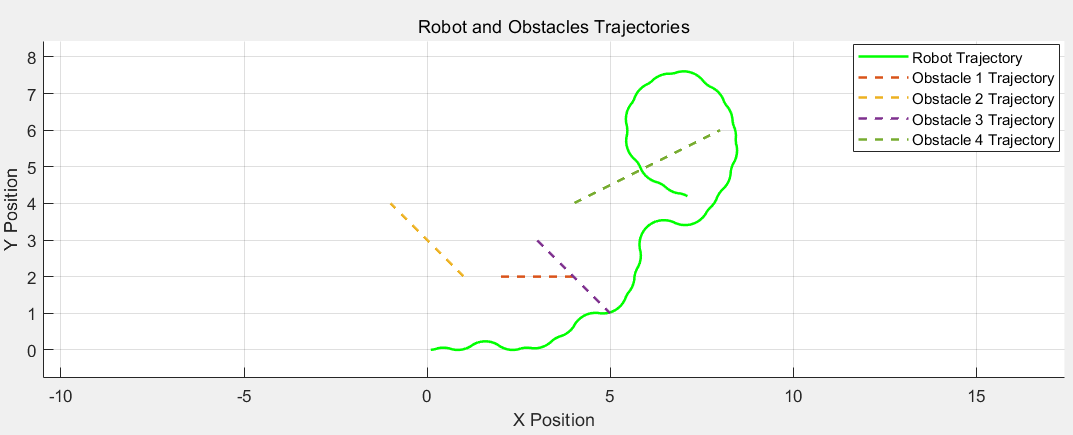
\includegraphics[width=0.8\textwidth]{5.png}
    \caption{Robot and Obstacles Trajectories}
    \label{FIG:5}
\end{figure}

\subsubsection{Temporal Evolution of Distances}

The robot-obstacle distance profiles over the 20-second simulation period are shown in Figure \ref{FIG:6}. Each curve corresponds to a specific obstacle, highlighting the robot's ability to maintain a minimum safety distance of \(2\,\text{m}\) throughout the test. The oscillatory patterns in the distance profiles reflect the robot's real-time responses to obstacle movements and interactions with multiple obstacles.

\begin{figure}[H]
    \centering
    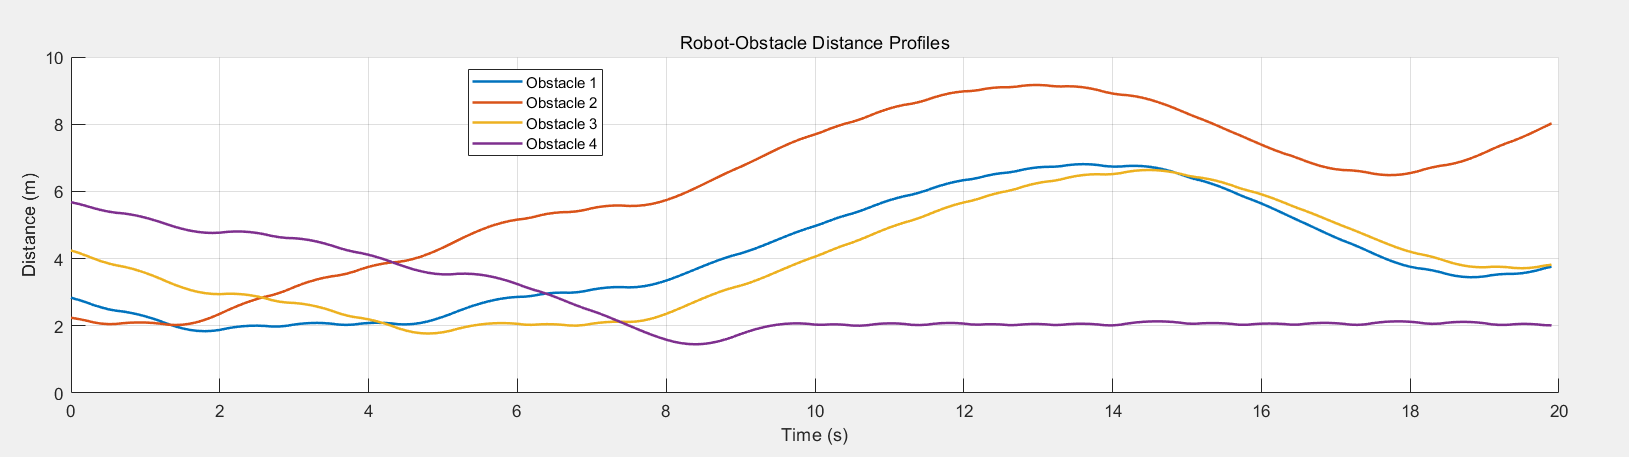
\includegraphics[width=0.8\textwidth]{6.png}
    \caption{Temporal Evolution of Robot-Obstacle Distances}
    \label{FIG:6}
\end{figure}

\subsubsection{Discussion}

The results validate the robustness of the SMC algorithm in environments with dynamic obstacles. The robot's trajectory demonstrates smooth transitions and efficient avoidance maneuvers, while the distance profiles confirm the maintenance of the safety threshold. This test highlights the capability of SMC to handle more complex and dynamic environments, laying the groundwork for future applications in real-world scenarios.

\subsection{Navigation to Target in a Static Obstacle Field}

In this test scenario, the initial position of the robot is set at $(0, 0)$, and the target point is located at $(5, 4)$. The environment contains three static obstacles with coordinates $(1, 1)$, $(2, 2)$, and $(4, 3)$, respectively. During path planning, the robot must navigate around the obstacles while maintaining a safety distance of $d_{\text{safe}} = 2$ and eventually reach the target point.

As shown in Figure \ref{FIG:7}, the green trajectory line represents the actual path taken by the robot, the red crosses indicate the positions of the obstacles, and the blue circle denotes the target point. The dashed circles are centered on the obstacles, with a radius equal to the adjusted triggering distance $d_{\text{safe}} - \varepsilon$. These dashed circles represent the influence zones of the obstacles. When the robot enters these zones, it activates the obstacle avoidance mode, adjusting its angular velocity $u$ using sliding mode control to change direction and avoid collisions. Once the robot exits these zones, it switches to the target-following mode, moving directly toward the target point.
\begin{figure}[H]
    \centering
    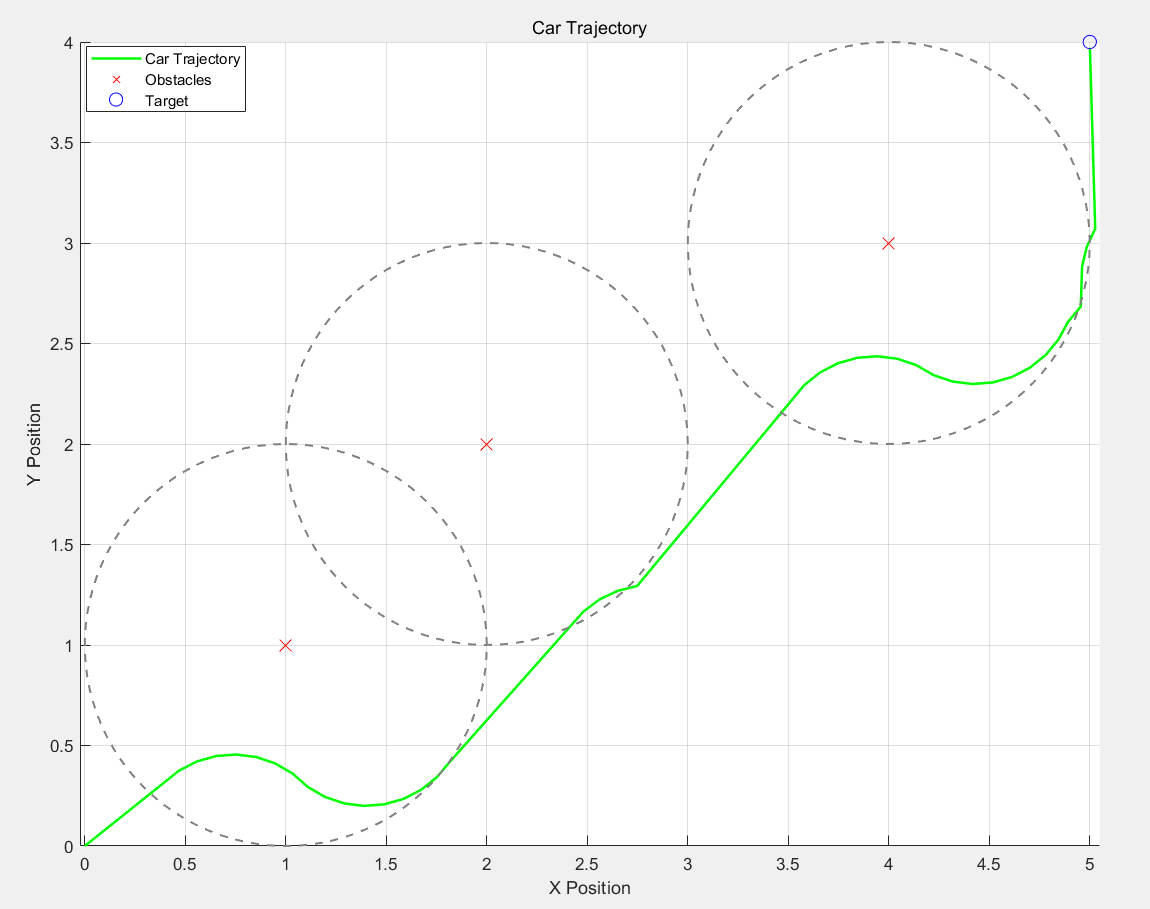
\includegraphics[width=0.8\textwidth]{7.png}
    \caption{Car Trajectory}
    \label{FIG:7}
\end{figure}

It is important to note that the obstacle avoidance and target-following mode switching logic implemented in this experiment is based on the goal-seeking algorithm proposed in Section 7 of the Reference \cite{Matveev2012}. 

The switching between the Proposed Guidance Law (PGL) and the Velocity Obstacle Approach (VOA)\cite{Fiorini1998} is the core logic for enabling the robot to navigate smoothly to the target. When the robot detects the nearest obstacle within a certain range, it calculates the distance $d_t$ to the closest obstacle and compares it to the threshold triggering distance $d_{\text{safe}} - \varepsilon$. Here, $d_{\text{safe}}$ represents the predefined safety distance, and $\varepsilon$ is an adjustable parameter that fine-tunes the triggering condition. Once $d_t \leq d_{\text{safe}} - \varepsilon$, the robot activates obstacle avoidance mode, during which sliding mode control is employed to regulate the robot's angular velocity $u$.

Sliding mode control uses the deviation $z = d_t - d_{\text{safe}}$ to compute the control law. If $|z| > \delta$, a proportional control $\chi_z = v^* \cdot \text{sign}(z)$ is applied to ensure rapid adjustments, where $v^*$ is the switching velocity determined by the algorithm parameters. Conversely, when $|z| \leq \delta$, a linear control $\chi_z = \gamma \cdot z$ is used, where $\gamma$ represents a constant gain. This hybrid control strategy ensures that the robot avoids obstacles efficiently while minimizing abrupt changes in direction.

When the robot exits the obstacle's influence zone, such that $d_t > d_{\text{safe}} - \varepsilon$, it switches to the target-following mode. In this mode, the robot calculates the direction angle $\theta_{\text{to target}}$ toward the target and moves along a straight line with a constant linear velocity $v$, aligning its heading angle $\theta$ with $\theta_{\text{to target}}$.

In practical operation, this algorithm demonstrates its efficiency in complex environments. By appropriately tuning the parameter $\varepsilon$, it achieves optimal path planning while avoiding obstacles, validating the applicability and effectiveness of the reference algorithm in scenarios with static obstacles.


\subsection{Navigation to Target in a Moving Obstacle Field}

This section will test the ability of the wheeled robot to avoid multiple moving obstacles and navigate to the target using the sliding mode control method. The settings for this scenario are as follows: the robot starts from an initial position of $(0, 0)$ and aims to reach a target located at $(3, 4)$, represented by a red hollow circle. The trajectory of the robot is shown in the figure \ref{FIG:8}.

\begin{figure}[H]
    \centering
    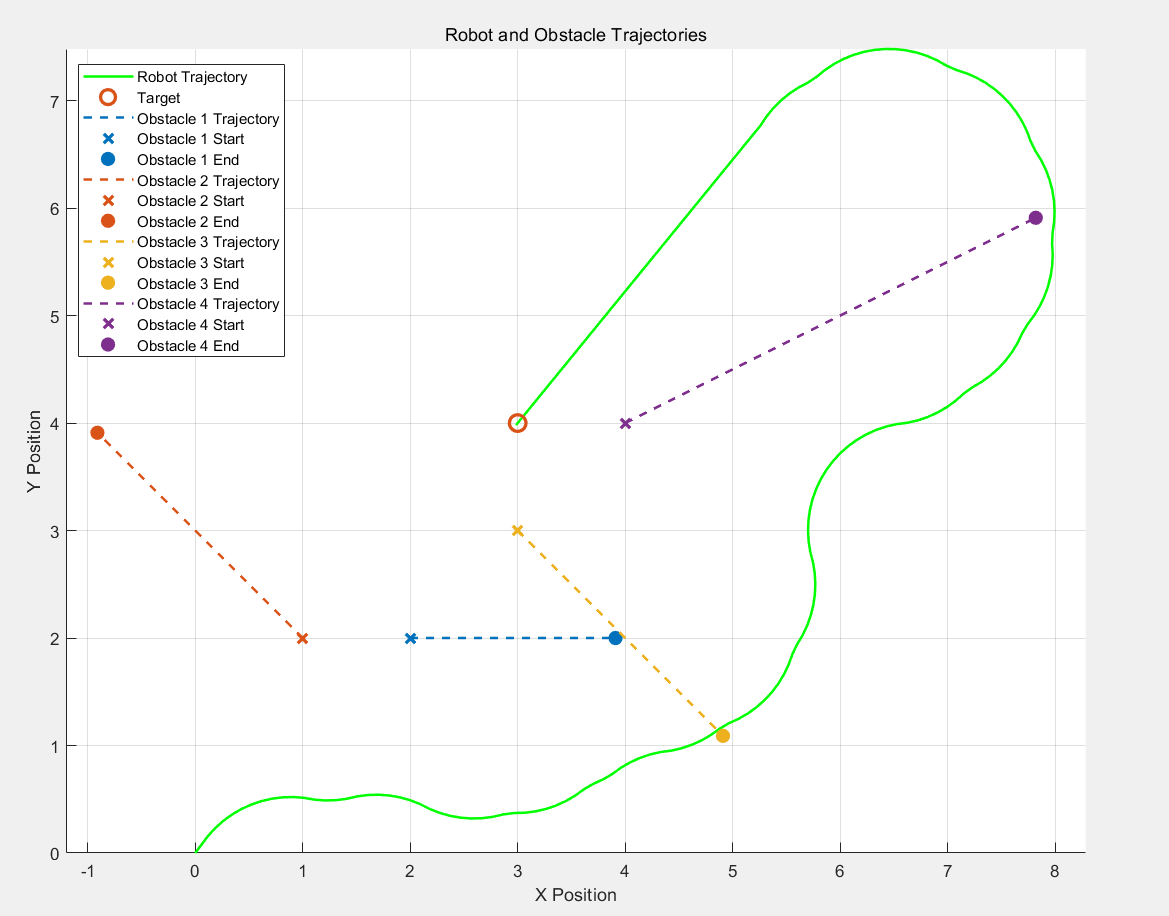
\includegraphics[width=0.8\textwidth]{8.png}
    \caption{Robot and Obstacles Trajectories}
    \label{FIG:8}
\end{figure}

\subsubsection{Parameter Settings}

The simulation parameters include a time step of $\Delta t = 0.1$ and a maximum simulation time of $t_{\text{max}} = 20$. The robot linear velocity is set to $v = 1.0$, with a maximum angular velocity of $u_{\text{max}} = 1.0$. For collision avoidance, a safe distance of $d_{\text{safe}} = 2.0$ is used. The sliding mode control parameters are $\gamma = 0.4$ and $\delta = 0.7$, and the proximity threshold to determine the target reach is $0.05$. 

The dynamic obstacles are initialized with specific properties, including their initial positions and velocities, as well as their trajectories, which are visualized in Figure 4.8. The initial positions and velocities are as follows: Obstacle 1 starts at position \((2.0, 2.0)\) with velocity \((0.1, 0.0)\), Obstacle 2 starts at position \((1.0, 2.0)\) with velocity \((-0.1, 0.1)\), Obstacle 3 starts at position \((3.0, 3.0)\) with velocity \((0.1, -0.1)\), and Obstacle 4 starts at position \((4.0, 4.0)\) with velocity \((0.2, 0.1)\). The trajectories of these obstacles, including their start and end points, are recorded as follows: Obstacle 1 travels from \((2.0, 2.0)\) to \((0.0, 2.0)\), Obstacle 2 from \((1.0, 2.0)\) to \((1.0, 4.0)\), Obstacle 3 from \((3.0, 3.0)\) to \((2.0, 2.0)\), and Obstacle 4 from \((4.0, 4.0)\) to \((6.0, 6.0)\).

\begin{figure}[H]
    \centering
    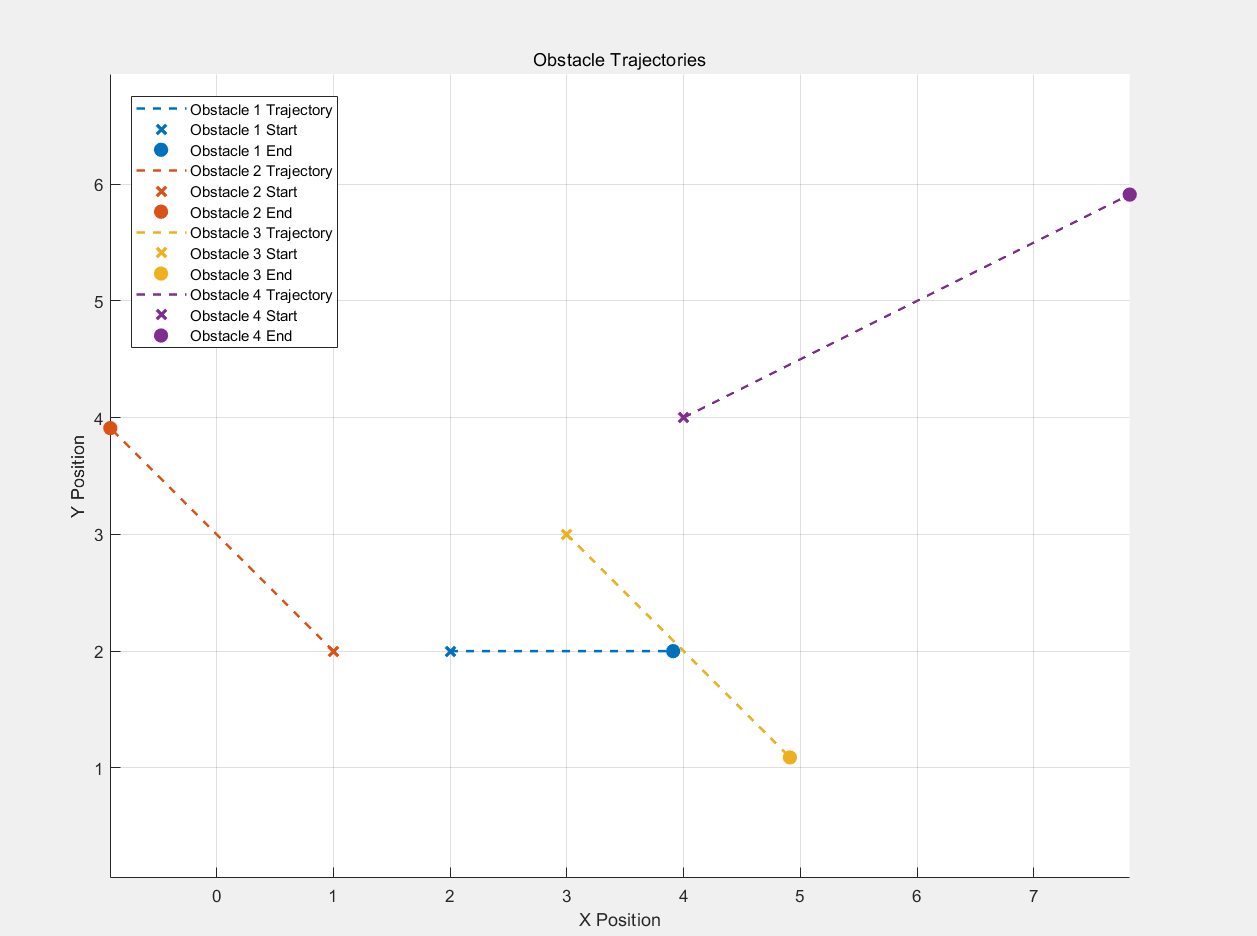
\includegraphics[width=0.8\textwidth]{9.png}
    \caption{Obstacles Trajectory}
    \label{FIG:9}
\end{figure}

\subsubsection{Simulation Results and Trajectory Analysis}

The robot's trajectory and obstacle avoidance behavior are analyzed in Figure~\ref{FIG:10}. When obstacles are distant from the robot, it moves directly toward the target along a straight line. However, as obstacles approach the safe distance threshold ($d_t \leq d_{\text{safe}}$), the robot's trajectory smoothly deviates to avoid collisions, showcasing the dynamic adjustments facilitated by the sliding mode control strategy. 


\begin{figure}[H]
    \centering
    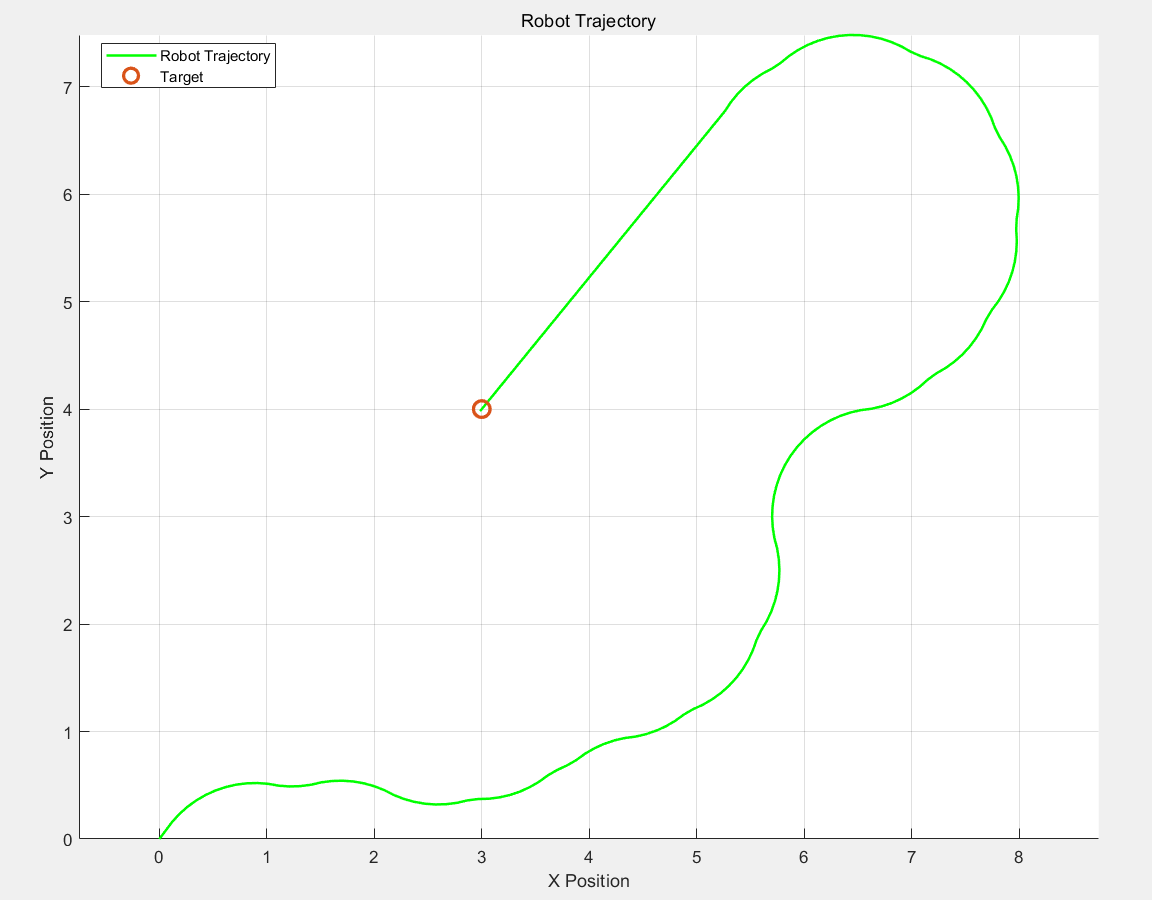
\includegraphics[width=0.8\textwidth]{10.png}
    \caption{Robot Trajectory}
    \label{FIG:10}
\end{figure}

The obstacle trajectories are visualized as dashed lines, with start and end points marked by “$\times$” and solid circles, respectively. For example, obstacle 2 exhibits vertical motion, while obstacle 4 moves diagonally away. These trajectory patterns confirm the accuracy of the initial velocity settings.
In the test scenario where the robot advances toward the target in the presence of dynamic obstacles, additional parameters need to be introduced to control the robot's trajectory to prevent collisions with unpredictable dynamic obstacles. The consideration of specific parameters refers to a series of inequalities mentioned in \cite{Matveev2012}. Next, I will list these inequality requirements one by one and calculate the relevant parameters for this scenario based on these formulas.

\subsubsection*{Parameter Selection and Calculation}

In the navigation and obstacle avoidance strategy, the parameters \(\varepsilon\), \(d_0\), and \(C\) must satisfy specific constraints to ensure system feasibility and safety. Additionally, the dynamic range of obstacles \(\mathcal{R}_{\text{max}}^{\text{av}}\), the robot’s turning radius \(R\), and the minimum obstacle distance \(d_{\text{obs}}\) are calculated to define these constraints. 

The dynamic range of obstacles is calculated as:
\begin{equation}
\mathcal{R}_{\text{max}}^{\text{av}} = \sqrt{(v_x \cdot t_{\text{max}})^2 + (v_y \cdot t_{\text{max}})^2},
\end{equation}
resulting in a maximum value of \(\mathcal{R}_{\text{max}}^{\text{av}} = 4.472\). The robot’s turning radius is determined as:
\begin{equation}
R = \frac{v}{u_{\text{max}}} = 0.5,
\end{equation}
and the minimum obstacle distance is constrained by:
\begin{equation}
d_{\text{obs}} > 2(R + \mathcal{R}_{\text{max}}^{\text{av}} + d_{\text{safe}}),
\end{equation}
yielding \(d_{\text{obs}} > 13.744\). 

For the parameter \(d_0\), the safe distance constraint requires:
\begin{equation}
d_0 > d_{\text{safe}} = 1.9,
\end{equation}
while the obstacle spacing constraint imposes:
\begin{equation}
d_0 < \frac{d_{\text{obs}}}{2} - (R + \mathcal{R}_{\text{max}}^{\text{av}}) = 2.028.
\end{equation}
To satisfy these bounds, \(d_0\) is chosen as \(2.0\). 

The constraint on \(\varepsilon\) is defined by:
\begin{equation}
\varepsilon < 2(R + \mathcal{R}_{\text{max}}^{\text{av}}) = 9.944,
\end{equation}
So \(\varepsilon = 0.2\) is selected. Finally:
\begin{equation}
C = d_0 + \varepsilon = 2.2,
\end{equation}
satisfying the condition:
\begin{equation}
2(R + \mathcal{R}_{\text{max}}^{\text{av}}) < C < \frac{d_{\text{obs}}}{2} - (R + \mathcal{R}_{\text{max}}^{\text{av}}).
\end{equation}


These parameter values ensure the robot operates safely and efficiently in the defined obstacle environment.


\subsubsection{Conclusion}

The simulation results, visualized in Figure~\ref{FIG:8}, demonstrate the effectiveness of the sliding mode control strategy in enabling the robot to navigate a dynamic, multi-obstacle environment. The robot successfully reaches its target while avoiding all obstacles, following an optimal path.


\subsection{Performance Metrics}

To quantitatively evaluate the effectiveness of the Sliding Mode Control (SMC) algorithm in navigation and obstacle avoidance, the following two performance metrics will be analyzed in the next section based on the results from the four test scenarios mentioned above.

The \textbf{Path Efficiency} metric evaluates the algorithm’s ability to optimize the robot’s trajectory. It is computed as the ratio of the actual distance traveled by the robot to the shortest possible path to the target. A value close to unity signifies that the robot follows an efficient trajectory with minimal deviations, while larger values indicate unnecessary detours caused by obstacle avoidance maneuvers.

The \textbf{Computation Time} evaluates the real-time feasibility of the SMC algorithm. This is determined by comparing the step size used during the simulation with the total step size. Computation time is critical for practical implementation in autonomous navigation systems and serves as an important measure of the algorithm's efficiency.

The evaluation of these metrics across all test scenarios allows for a detailed understanding of the strengths and limitations of the SMC algorithm. By analyzing the trajectory, obstacle distances, and computational demands, this study offers a comprehensive framework to assess the algorithm’s performance in environments with varying complexity and obstacle dynamics. These findings will be discussed in the subsequent \textit{Discussion} chapter, providing insights into the controller’s adaptability and reliability.

\chapter{Discussion}

This chapter provides an in-depth analysis of the experimental results, focusing on two performance metrics demonstrated by the robot under the SMC control strategy:  path efficiency and computation time. Each metric is evaluated in detail to analyze the strengths and limitations of the Sliding Mode Control (SMC) algorithm in navigation and obstacle avoidance tasks.


\section{Path Efficiency}

Path efficiency is an important metric for evaluating the performance of the Sliding Mode Control (SMC) algorithm. Ideally, the robot should follow the shortest path from the starting point to the target. However, due to the presence of obstacles, different control strategies are employed to guide the robot in avoiding obstacles and reaching the target. The path lengths resulting from different strategies vary. This section provides a comparative analysis of the path length achieved by the SMC strategy against the shortest possible path.

As shown in Figure~\ref{fig:shortest_path}, the shortest path is a straight line connecting the start and target positions. Its length can be calculated using the following formula:
\begin{equation}
L_{\text{shortest}} = \sqrt{(x_{\text{goal}} - x_{\text{start}})^2 + (y_{\text{goal}} - y_{\text{start}})^2}
\end{equation}
where $(x_{\text{start}}, y_{\text{start}})$ and $(x_{\text{goal}}, y_{\text{goal}})$ represent the coordinates of the start and target positions, respectively. In this experiment, the start position is $(0, 0)$, and the target position is $(5, 4)$. Substituting these values yields:
\begin{equation}
L_{\text{shortest}} = \sqrt{(5 - 0)^2 + (4 - 0)^2} = \sqrt{25 + 16} = 6.4 \, \text{units}
\end{equation}

\begin{figure}[ht]
    \centering
    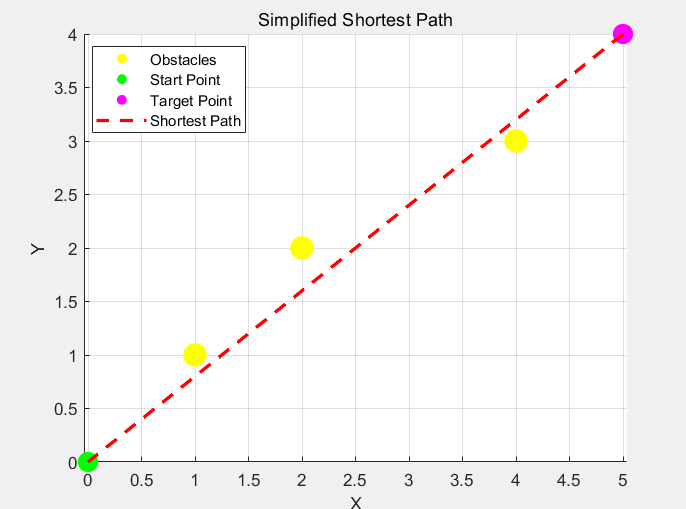
\includegraphics[width=0.6\textwidth]{image/12.PNG}
    \caption{Shortest path connecting the start and target positions}
    \label{fig:shortest_path}
\end{figure}

In contrast, the actual path length is calculated by summing the distances between successive points in the robot's trajectory. As illustrated in Figure~\ref{FIG:7}, the robot's trajectory, generated by the SMC algorithm, avoids obstacles and ultimately reaches the target. The trajectory is recorded as a sequence of discrete points $(x_1, y_1), (x_2, y_2), \dots, (x_n, y_n)$, and the actual path length is computed as:
\begin{equation}
L_{\text{actual}} = \sum_{i=1}^{n-1} \sqrt{(x_{i+1} - x_i)^2 + (y_{i+1} - y_i)^2}
\end{equation}
Using this formula and the recorded trajectory, the actual path length was determined to be:
\begin{equation}
L_{\text{actual}} = 7.6 \, \text{units}
\end{equation}

Path efficiency is defined as the ratio of the shortest path length to the actual path length:
\begin{equation}
\text{Path Efficiency} = \frac{L_{\text{shortest}}}{L_{\text{actual}}}
\end{equation}
Substituting the values obtained:
\begin{equation}
\text{Path Efficiency} = \frac{6.4}{7.6} \approx 0.842
\end{equation}

The results demonstrate that the SMC algorithm effectively maintains high path efficiency while avoiding obstacles. Although the actual path length is approximately \(18.75\%\) longer than the shortest path, this deviation is primarily due to the robot's detours to maintain a safe distance from obstacles. For most of the navigation process, the robot aligns its movement towards the target, achieving a reasonable balance between goal-directed behavior and collision avoidance.

\section{Computation Time}

Computation time is a critical metric for evaluating the real-time performance of navigation algorithms. This section presents the computation time required to complete the navigation tasks in both scenarios.

\subsubsection{Static Obstacle Navigation}

In the static obstacle scenario, the robot starts from the initial position (0, 0) and navigates to the target position (5, 4). The simulation parameters are set with a time step \(dt = 0.1\) and a maximum simulation time of 20 seconds. The total number of iterations can be calculated using the following formula:
\[
N = \frac{t_{\text{max}}}{dt} = \frac{20}{0.1} = 200 \, \text{steps}
\]

During navigation, the robot avoids obstacles while gradually approaching the target. According to the real-time display outputs, the robot reaches the target at step 77 with the following observations (Figure~\ref{fig:static_output}):

\begin{figure}[ht]
    \centering
    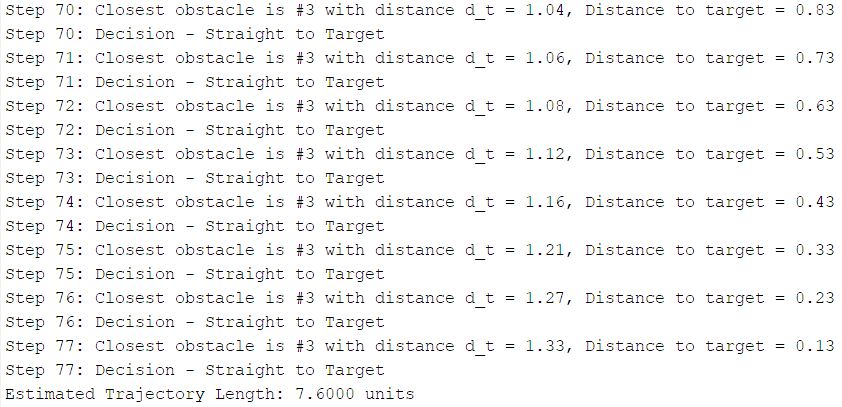
\includegraphics[width=0.8\textwidth]{13.png}
    \caption{Real-time outputs for the static obstacle scenario}
    \label{fig:static_output}
\end{figure}

In step 77, the robot is 1.33 units from the closest obstacle (Obstacle \#3) and 0.13 units from the target. At this point, the robot determines that it can move straight toward the target and completes the task. The total trajectory length is approximately \(7.600 \, \text{units}\). The task is completed in \(T_{\text{total}} = 7.7 \, \text{seconds}\). Figure~\ref{fig:static_output} illustrates the task completion process in the static obstacle scenario.


\subsubsection{Dynamic Obstacle Navigation}

In the dynamic obstacle scenario, the robot starts at \((0, 0)\) and navigates to a dynamic target located at \((3, 4)\). Dynamic obstacles move with constant velocity, increasing the complexity of the navigation task. The simulation parameters are the same as in the static scenario, with \(dt = 0.1\), \(t_{\text{max}} = 20\) seconds and 200 total steps.

The robot adjusts its path multiple times to avoid moving obstacles while gradually approaching the dynamic target. The real-time display outputs for steps 195 to 200 are as follows (Figure~\ref{fig:dynamic_output}):

\begin{figure}[ht]
    \centering
    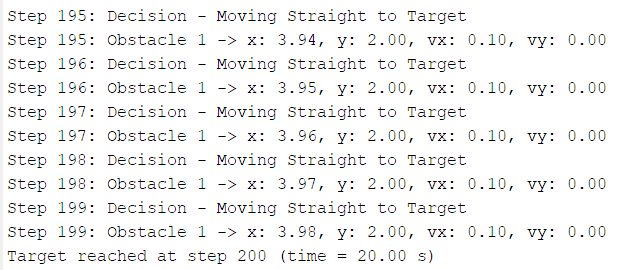
\includegraphics[width=0.8\textwidth]{14.png}
    \caption{Real-time outputs for the dynamic obstacle scenario}
    \label{fig:dynamic_output}
\end{figure}

In step 199, obstacle \#1 is located at \((3.98, 2.00)\) with a speed of \((v_x = 0.10, v_y = 0.00)\). The robot successfully reaches the target at step 200, completing the task in \(T_{\text{total}} = 20.0 \, \text{seconds}\). Figure~\ref{fig:dynamic_output} illustrates the task completion process in the dynamic obstacle scenario.


\subsubsection{Comparison and Discussion}

The comparison between static and dynamic obstacle scenarios reveals the impact of obstacle movement on navigation performance. In the dynamic scenario, the robot requires more adjustments to avoid moving obstacles, resulting in a longer task completion time. Table~\ref{tab:comparison} summarizes the task completion times and critical decision steps for both scenarios.


\begin{table}[H]
    \centering
    \caption{Comparison of static and dynamic obstacle navigation scenarios}
    \label{tab:comparison}
    \centering
    \begin{tabular}{|l|c|c|c|}
        \hline
        \textbf{Scenario} & \textbf{Total Step} & \textbf{Target Position} & \textbf{Decision Steps} \\ \hline
        Static Obstacle Navigation & 77 & (5, 4) & Step 77 \\ \hline
        Dynamic Obstacle Navigation & 200 & (3, 4) & Steps 200 \\ \hline
    \end{tabular}
\end{table}



\subsubsection{Summary}

The comparison shows that the SMC algorithm achieves a favorable computing time in the static obstacle environment. However, in the dynamic obstacle environment, the completion time significantly increases, reaching the maximum simulation duration. This increase in completion time is mainly due to frequent path adjustments and obstacle avoidance decisions in the dynamic obstacle environment.
\chapter{Conclusion}

The experiments demonstrate that the SMC algorithm exhibits high robustness in maintaining collision-free trajectories, even in challenging environments. In the static obstacle scenario, the wheeled robot achieved a Path Efficiency of 0.842, with a total computation time of 7.7 seconds, showcasing the algorithm's efficiency in static obstacle environments. In the dynamic obstacle scenario, the total computation time increased to 20 seconds, with unavoidable trajectory oscillations caused by frequent path switching. Nevertheless, the algorithm successfully avoided moving obstacles and reached the target. These results validate the adaptability of the SMC algorithm in handling both static and dynamic obstacles.

\section*{Performance Summary}

The experiments demonstrated that the SMC algorithm achieves high robustness in maintaining collision-free trajectories even in challenging environments. In the static obstacle scenario, the robot completed the navigation task with a success rate of 100\% and a total computation time of \(T_{\text{total}} = 7.7 \, \text{seconds}\), showcasing the algorithm’s efficiency in simpler environments. Similarly, in the dynamic obstacle scenario, the algorithm effectively avoided moving obstacles and successfully reached the target, albeit with a longer computation time of \(T_{\text{total}} = 20.0 \, \text{seconds}\) due to frequent path adjustments. These results confirm the adaptability of the SMC algorithm in handling both static and dynamic obstacles.

\section*{Real-time Feasibility}

The computation time analysis underscores the real-time applicability of the SMC algorithm. While the algorithm's response time remained within acceptable limits for dynamic scenarios, its reliance on frequent trajectory recalculations under dynamic conditions increased computational overhead. Optimizing this aspect could further enhance the algorithm’s practical deployment in real-world applications.

\section*{Challenges and Limitations}

In conclusion, this study highlights the effectiveness of the SMC algorithm for collision-free navigation in both static and dynamic environments. By addressing the identified limitations, the SMC algorithm can be further refined to achieve greater efficiency and reliability, contributing to the advancement of autonomous robotic navigation systems in complex real-world scenarios.


\cite{Liu2012}
\cite{Hoy2015}
\cite{Matveev2012}
\cite{Fiorini1998}
\cite{Mayne2014}
\cite{Falcone2016}
\cite{Edwards2000}
\cite{Sarkar2009}
\cite{Fiorini1998}
\cite{Bareiss2015}
\cite{Kim2000}
\cite{Ge2000}
\cite{Lumelsky1991}
\cite{Turpin2014}
\cite{Dunbar2006}

\printbibliography % 打印参考文章列表
\end{document}

